\begin{Problem}
	Gegeben sei die Relation $\sim\subseteq (\R^2 \ \{0\}) \times  (\R^2 \ \{O\})$ mit $x\sim y$ genau dann, wenn es eine Gerade $L \subseteq \R^2$ gibt, die $0$, $x$ und $y$ enthält.

	\begin{parts}
		\item Bestimmen Sie alle $y \in \R^2 \backslash \{(0, 0)\}$ mit $(0, 1) \sim y$ bzw. $(1, 0) \sim y$ und skizzieren Sie die beiden Mengen in einem geeigneten Koordinatensystem.
		\item Begründen Sie, dass $\sim$ eine Äquivalenzrelation ist.
		\item Bleibt $\sim$ auch dann eine Äquivalenzrelation, wenn man sie als Relation in $\R^2$ betrachtet?
	\end{parts}
\end{Problem}
\begin{proof}
	\begin{parts}
	\item Eine Gerade hat den Form
		\[
		\left\{ (x_1,x_2)\in\R^2|a_1x_1+a_2x_2=b \right\} 
		.\] 
		Weil $(0,0)$ in der Gerade ist, gilt $b=0$. F\"{u}r die zwei F\"{a}lle:
		\begin{enumerate}[label=(\roman*)]
			 \item $(0,1)$ ist in der Gerade. Es gilt dann $a_2=0, a_1\in \R$. Die Gleichung der Gerade ist dann $x_1=0$, oder alle Punkte des Forms $(0,y), y\in \R$.

			 \item $(1,0)$ ist in der Gerade. Es gilt dann $a_1=0, a_2\in \R$. Die Gerade enthält ähnlich alle Punkte des Forms $(x,0), x\in \R$.
		\end{enumerate}
		
		
		\begin{center}
			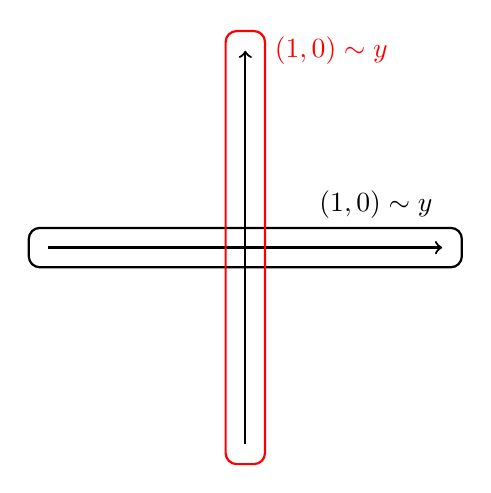
\begin{tikzpicture}[scale=2.5]
				\draw[thick, ->] (-1,0) -- (1,0);
				\draw[thick, ->] (0,-1) -- (0,1);
				\draw[thick, rounded corners] (-1.1,-0.1) rectangle (1.1,0.1);
				\draw (1,0.1) node[anchor=south east] {$(1,0)\sim y$};
				\draw[thick, red,rounded corners] (-0.1,-1.1) rectangle (0.1,1.1);
				\draw[red] (0.1,1) node[anchor=west] {$(1,0)\sim y$};5
			\end{tikzpicture}
		\end{center}
	\item 
		\begin{enumerate}[label=(\roman*)]
			\item $x\sim x$ (Reflexivität)

				Es gibt immer eine Gerade zwischen $0$ und $x$. Eine solche Gerade enthält $x$ per Definition.

			\item $x\sim y \iff y\sim x$ (Symmetrie)

				Es gibt eine Gerade, die $0$, $x$ und $y$ enthält. Deswegen gilt die beide Richtung der Implikationen.

			\item $x\sim y$ und $y\sim z\implies x\sim z$ (Transitivität)

				Es gibt eine Gerade zwischen $0,x$ und $y$, und eine Gerade zwischen $0, y$ und $z$. Weil die beide Geraden zwischen $y$ geht, sind die Geraden gleich, und enthält $x$ und $z$, daher $x\sim z$.
		\end{enumerate}
		\item Nein. $(1,0)\sim (0,0), (0,1)\sim (0,0)$, aber $(1,0)\sim (0,1)$ stimmt nicht.
	\end{parts}
\end{proof}

\begin{Problem}
	Es sei $f: \R^3\to \R^2$ mit $(x_1, x_2, x_3) \to (x_1, x_2)$, $s$ die Spiegelung in $\R^2$, $T : \R^2 \to \R^2$ die Translation um $(1, 0)$ und $em : \R^2 \to \R^3$ die Einbettung.
	\begin{parts}
		\item 	Bilden Sie die Verkettungen $f \circ em, em \circ f , s \circ f , T \circ s, s \circ T$ und $em \circ s$. Geben Sie dabei jeweils Argumentmenge, Zielmenge und Zuordnungsvorschrift an.
		\item  Untersuchen Sie die Funktionen aus der vorherigen Teilaufgabe auf Surjektivit\"{a}t, Injektivit\"{a}t bzw. Bijektivit\"{a}t.
		\item  Sei $F = em\circ T \circ s\circ f$. Bestimmen und skizzieren Sie das Bild bzw. Urbild von $[0,1]\times [-1,1]\times [0,2]$ unter  $F$.
	\end{parts}
\end{Problem}

\begin{proof}
	\begin{parts}
		\item
		\begin{enumerate}[label=(\roman*)]
			\item $f\circ em$
			
			
			Argumentmenge: $\R^2$
			
			Zielmenge: $\R^2$
			
			Zuordnungsvorschrift:  $(x_1,x_2)\to (x_1,x_2)=\text{Id}_{\R^2}$
			
			\item $em \cdot f$
			
			Argumentmenge + Zielmenge:  $\R^3$ 
			
			Zuordnungsvorschrift: $(x_1,x_2,x_3)\to (x_1,x_2,0)$ 
			
			\item $s\cdot f$ 
			
			Argumentmenge: $\R^3$ 
			
			Zielmenge: $\R^2$ 
			
			Zuordnungsvorschrift: $(x_1,x_2,x_3)\to (x_2,x_1)$
			\item $em\circ s$
			
			Argumentmenge:  $\R^2$
			
			Zielmenge:  $\R^3$
			
			Zuordnungsvorschrift:  $(x_1,x_2)\to (x_2,x_1,0)$
		\end{enumerate}
		\item
		\begin{enumerate}[label=(\roman*)]
			\item $f\circ em$
			
			Surjektive, injektive und auch bijektive
			
			\item $em\circ f$ 
			
			Injektiv, aber nicht surjektiv (und deswegen nicht Bijektiv)
			
			\item $s\circ f$ 
			
			Surjektive, aber nicht injektiv
			
			\item $em\circ s$ 
			
			Injektiv, aber nicht surjektiv
		\end{enumerate}
	\item \noindent \\


		\begin{minipage}{0.4\textwidth}
			Bild: $[0,2]\times [0,1]\times \left\{ 0 \right\} $ 
			\begin{center}
				$z=0$ Ebene


				\begin{tikzpicture}[scale=2]
					\draw[thick,->] (-0.1,0) -- (2.5,0);
					\draw[thick,->] (0,-0.1) -- (0,1.5);
					\fill[pattern=north east lines](0,0) rectangle (2,1);
					\draw[thick] (0,0) rectangle (2,1);
					\draw (2,0) node[anchor=north] {$2$};
					\draw (0,1) node[anchor=east] {$1$};
					\draw (0,-0.1) node[anchor=west] {$0$};
					\draw (-0.1,0) node[anchor=south] {$0$};
				\end{tikzpicture}
			\end{center}
		\end{minipage}
		\begin{minipage}{0.4\textwidth}
			Urbild: $[0,1]\times [-2,0]\times \R$
			 \begin{center}
				 $z=0$ Ebene


					\begin{tikzpicture}
						\draw[thick,->] (0,-2.5) -- (0,0.2);
					\draw[thick,->] (-0.1,0) -- (1.5,0);
					\filldraw[pattern = north east lines, thick] (0,-2) rectangle (1,0);
					\draw (0,-2) node[anchor=east] {$-2$};
					\draw (-0.1,0) node[anchor=east] {$0$};
					\draw (1,0) node[anchor=south] {$1$};
				\end{tikzpicture}
			\end{center}
		\end{minipage}
	\end{parts}
\end{proof}
\begin{Problem}
		Es sei $M$ eine beliebige, nichtleere Menge und $f : M \to M$ eine Abbildung. Wir definieren induktiv $f^0 := id$ und f\"{u}r $k \in \N f^k := f \circ f^{k-1}$.

		\begin{parts}
		\item Zeigen Sie: $f^{k+l} = f^k \circ f^l$ f\"{u}r alle $k, l \in \N_0$
		\item Zeigen Sie: Gibt es $k_0 \in \N \cup \{0\}$ und $l \in \N$ mit $f^{k_0+l} = f^{k_0}$, dann gilt $f^{k+l} = f^k$ f\"{u}r alle $k \in \N_0$ mit $k\ge k_0$.
		\item Geben Sie eine Funktion $f : \{1, 2, 3, 4, 5\} \to \{1, 2, 3, 4, 5\}$ an, f\"{u}r die $f^1\neq f^3$, aber $f^{k+2} = f^k$ f\"{u}r alle $k\ge 2$ gilt. Begr\"{u}nden Sie, dass Ihre Funktion diese Eigenschaft hat.
		\end{parts}
\end{Problem}
\begin{proof}
	\begin{parts}
	\item Wir beweisen es per Induktion auf $k$. F\"{u}r $k=1$ gilt es per Definition (es wird in der Frage gegeben). Jetzt nehme an, dass es f\"{u}r ein beliebige $k\in\N$ gilt. 
	
		Es gilt dann:
		\begin{align*}
			f^{(k+1)+l}=&f\circ f^k\circ f^l\\
			=& f^{k+1}\circ f^l
		\end{align*}
		Deswegen gilt es auch f\"{u}r $k+1$, und daher f\"{u}r alle $k\in \N$.
	\item Sei $k=k_0+k'$. Es gilt
		\[
			f^{k+l}=f^{k_0+k'+l}=f^{k_0}=f^{k_0+k'}=f^k
		.\] 
	\item Sei $f$ definiert durch
		\begin{align*}
			f(1)=&1\\
			f(2)=&1\\
			f(3)=&2\\
			f(4)=&1\\
			f(5)=&4
		\end{align*}
		Es gilt dann
		\begin{center}
			\begin{tabular}{cccccc}
				\toprule
				x & $f^1(x)$ & $f^2(x)$ & $f^3(x)$ & $f^4(x)$ & $f^5(x)$\\\midrule
				1 & 1 & 1 & 1 & 1 & 1\\\midrule
				2 & 1 & 1 & 1 & 1 & 1\\\midrule
				3 & 2 & 1 & 1 & 1 & 1\\\midrule
				4 & 1 & 1 & 1 & 1 & 1\\\midrule
				5 & 4 & 1 & 1 & 1 & 1\\\bottomrule
			\end{tabular}
		\end{center}
		$f^1\neq f^3$, weil $f^1(3)\neq f^3(3)$. Aber $f^k(x)=1\forall k \in \left\{ 1,2,3,4,5 \right\} , k\ge 2$. Daher ist $f^{k+2}=f^k, k\ge 2$.\qedhere
	\end{parts}
\end{proof}
\begin{Problem}
	Es seien $M, N$ Mengen, $m, n$ nat\"{u}rliche Zahlen und die Abbildungen $f : M \to \{1, 2, 3, \dots , m\}, g : N \to \{1, 2, 3,\dots , n\}$ bijektiv. Finden Sie eine nat\"{u}rliche Zahl $k$ und eine bijektive Abbildung $F : M \times  N \to \{1, 2, 3, \dots , k\}$.
\end{Problem}
\begin{proof}
	$k=nm$, und
	\[
	F(a,b)=a+(b-1)m
	.\] 
	Das ist bijektiv. Sei $x\in\left\{ 1,2,\dots,nm \right\} $. Es existiert eindeutige Zahlen $p,q\in\N$, so dass
	\[
	x=pm+q, q<m
	.\] 
	Falls $q=0$, sei $b=p,a=m$. Sonst definiert man $b=p+1,a=m$. Per Definition ist $a\in \left\{ 1,2,3,\dots,m \right\} $. Außerdem ist $1\le b\le n$, weil $p\le k / m=n$ ($n$ teilt $k=mn$).
\end{proof}
